% =====================================================================
% thesis.tex — Vietnamese Toxic Comment Detection on Social Media Using NLP Models
%
% Compile with XeLaTeX or LuaLaTeX (Unicode-native; handles Vietnamese cleanly).
% Sequence:
%     xelatex thesis.tex
%     biber thesis    (or bibtex thesis if you prefer)
%     xelatex thesis.tex
%     xelatex thesis.tex
%
% If your school requires pdflatex, swap fontspec/polyglossia for
% inputenc(utf8) + fontenc(T5) + babel(vietnamese,english).
% =====================================================================

\documentclass[a4paper,12pt,oneside]{report}

% ---- Encoding & fonts (XeLaTeX path) --------------------------------------
\usepackage{fontspec}
\usepackage{polyglossia}
\setdefaultlanguage{english}
\setotherlanguage{vietnamese}
\setmainfont{Latin Modern Roman}
\setmonofont{Latin Modern Mono}[Scale=0.9]

% ---- Layout ---------------------------------------------------------------
\usepackage[margin=2.8cm]{geometry}
\usepackage{setspace}
\onehalfspacing
\usepackage{microtype}
\usepackage{parskip}

% ---- Math, tables, figures ------------------------------------------------
\usepackage{amsmath, amssymb}
\usepackage{booktabs}
\usepackage{multirow}
\usepackage{array}
\usepackage{graphicx}
\usepackage{subcaption}
\usepackage{float}
\graphicspath{{../results/figures/}}

% ---- Code listings --------------------------------------------------------
\usepackage{listings}
\usepackage{xcolor}
\definecolor{codegray}{rgb}{0.95,0.95,0.95}
\lstset{
  backgroundcolor=\color{codegray},
  basicstyle=\ttfamily\footnotesize,
  breaklines=true,
  frame=single,
  numbers=left,
  numberstyle=\tiny\color{gray},
  showstringspaces=false,
}

% ---- Hyperref (load last) -------------------------------------------------
\usepackage[hidelinks]{hyperref}
\usepackage{cleveref}

% ---- Bibliography ---------------------------------------------------------
\usepackage[backend=biber, style=numeric, sorting=nyt]{biblatex}
\addbibresource{references.bib}

% =====================================================================
% TITLE PAGE METADATA
% =====================================================================
\newcommand{\thesistitle}{Vietnamese Toxic Comment Detection\\ on Social Media Using NLP Models}
\newcommand{\thesisauthor}{<YOUR NAME>}
\newcommand{\thesisid}{<STUDENT ID>}
\newcommand{\thesissupervisor}{<SUPERVISOR NAME>}
\newcommand{\thesisuniversity}{<UNIVERSITY NAME>}
\newcommand{\thesisfaculty}{<FACULTY / DEPARTMENT>}
\newcommand{\thesisyear}{2026}

\title{\thesistitle}
\author{\thesisauthor}
\date{\thesisyear}

% =====================================================================
\begin{document}

% ---------------------------------------------------------------------
% TITLE PAGE
% ---------------------------------------------------------------------
\begin{titlepage}
\centering
{\large \thesisuniversity \par}
{\large \thesisfaculty \par}
\vspace{2.5cm}
{\Huge \bfseries \thesistitle \par}
\vspace{1.5cm}
{\Large Graduation Thesis \par}
\vspace{3cm}
\begin{tabular}{rl}
\textit{Author:}     & \thesisauthor\ (\thesisid) \\[4pt]
\textit{Supervisor:} & \thesissupervisor \\
\end{tabular}
\vfill
{\large \thesisyear \par}
\end{titlepage}

% ---------------------------------------------------------------------
% ABSTRACT
% ---------------------------------------------------------------------
\chapter*{Abstract}
\addcontentsline{toc}{chapter}{Abstract}

% TODO: tighten to 150-250 words after the rest of the thesis is final.
We study three-class toxic comment classification (CLEAN / OFFENSIVE / HATE)
on Vietnamese social media using the ViHSD dataset~\cite{luu2021vihsd}.
We compare a tuned Logistic-Regression baseline with character n-gram
features, a 2-layer BiLSTM initialised with PhoW2V~\cite{nguyen2020phow2v}
word embeddings, and a fine-tuned PhoBERT-base-v2~\cite{nguyen2020phobert}
transformer. PhoBERT achieves the best test macro-F1 of \textbf{0.6618},
improving over the LR champion (0.6183) by +0.0435 absolute. Through a
two-phase error analysis on the test set, we find that
(i)~all three architectures share a near-constant
$\sim$30--34\% OFFENSIVE--to--CLEAN false-negative rate, indicating an
\emph{annotation ceiling} rather than a model-capacity gap;
(ii)~the popular ``short comments are hardest'' hypothesis is inverted on
ViHSD --- short comments are easiest (F1$\approx$0.71) while long comments
collapse the OFFENSIVE class to F1$\approx$0.03;
(iii)~PhoBERT is over-confident
(ECE = 0.106) and thus its raw softmax is unsafe as an auto-moderation
threshold. We propose a three-tier failure framework
(\emph{fixable / model-improvable / fundamentally hard}) that prioritises
re-annotation over more model capacity as the highest-leverage
improvement.

\textbf{Keywords:} hate speech detection, Vietnamese NLP, ViHSD, PhoBERT,
BiLSTM, error analysis, annotation noise.

% ---------------------------------------------------------------------
% TOC
% ---------------------------------------------------------------------
\tableofcontents
\listoffigures
\listoftables

% =====================================================================
\chapter{Introduction}
\label{ch:intro}

\section{Background and Motivation}
% TODO: 3-4 paragraphs. Suggested points (expand to prose):
%   * Vietnam's social media penetration (~73\% of population, ~77M users on
%     Facebook/TikTok/Zalo as of 2024). Cite a public statistics source.
%   * Toxic content creates platform-policy, mental-health, and legal risk;
%     manual moderation does not scale.
%   * Automated toxic-comment classification is well-studied in English
%     (Davidson 2017, Founta 2018) but Vietnamese has unique surface
%     properties --- diacritics, no whitespace word delimiter, heavy
%     teen-code obfuscation --- that prevent direct transfer of English
%     models.
%   * Hence the need for Vietnamese-specific evaluation on a Vietnamese
%     benchmark.

\section{Problem Statement}
We address \emph{three-class} toxic comment classification on Vietnamese
social-media text. Given a comment $x$, the model predicts a label
$y \in \{$\textsc{Clean}, \textsc{Offensive}, \textsc{Hate}$\}$,
where \textsc{Offensive} covers personal insults / abuse and \textsc{Hate}
covers attacks targeting a protected group (gender, region, ethnicity,
religion). The boundary between \textsc{Offensive} and \textsc{Hate}
is intentionally narrow in the ViHSD annotation guidelines and is, as we
show in Chapter~\ref{ch:errors}, a major source of irreducible label noise.

Vietnamese-specific challenges include:
\begin{itemize}
  \item \textbf{Word segmentation}: whitespace separates syllables, not
        words --- ``h\^om nay'' (two syllables) is one word ``h\^om\_nay''
        only after segmentation by tools such as \texttt{underthesea}.
  \item \textbf{Teen code / obfuscation}: explicit profanity is routinely
        rewritten (\texttt{vcl} for \emph{v\~ai c\'a l\d{o}n},
        \texttt{\dj\d{a}u m\'a} as a softened spelling of \emph{\dj m}) to
        evade keyword filters.
  \item \textbf{Code-switching}: English profanity intermixes with
        Vietnamese in younger demographics.
  \item \textbf{Severe class imbalance} (Section~\ref{sec:imbalance}).
\end{itemize}

\section{Objectives}
\begin{enumerate}
  \item Build, train, and evaluate models spanning three paradigms:
        traditional ML (LR, NB, SVM with BoW / TF-IDF / char n-grams),
        deep learning (BiLSTM with PhoW2V word embeddings), and a
        fine-tuned transformer (PhoBERT-base-v2).
  \item Establish a fair 3-way comparison on the ViHSD test set under a
        strict ``touch test once'' protocol.
  \item Conduct an in-depth error analysis (quantitative + qualitative)
        to localise \emph{where} and \emph{why} the champion still fails.
  \item Propose a deployment-oriented framework that separates fixable,
        model-improvable, and fundamentally hard failure modes.
\end{enumerate}

\section{Contributions}
\begin{itemize}
  \item A reproducible end-to-end pipeline (Weeks 1--5 of this project,
        single git repository, fixed \texttt{random\_state=42}) over the
        ViHSD benchmark spanning Logistic Regression to PhoBERT.
  \item Empirical evidence that, for Vietnamese hate speech,
        \emph{character n-gram} features dominate word n-grams in the LR
        family (Section~\ref{sec:lr-results}) --- a non-obvious finding
        given that Vietnamese segmentation is a heavy preprocessing step.
  \item A \textbf{three-tier failure framework} (annotation /
        implicit-contextual / surface) derived from manually tagging 98
        failure cases across eight error categories
        (Chapter~\ref{ch:errors}).
  \item Quantification of the \emph{annotation ceiling}: a $\sim$30--34\%
        OFFENSIVE-to-CLEAN false-negative rate that is essentially
        invariant across LR, BiLSTM, and PhoBERT, implying that further
        modelling will not move the needle without re-annotation.
  \item A counter-intuitive finding that short comments are
        \emph{easiest} on ViHSD; the OFFENSIVE F1 drops from
        $\sim$0.60 to $\sim$0.03 as comment length grows.
\end{itemize}

\section{Thesis Structure}
Chapter~\ref{ch:related} surveys prior work on hate-speech detection,
Vietnamese NLP, and PhoBERT.
Chapter~\ref{ch:dataset} describes the ViHSD dataset and its idiosyncrasies.
Chapter~\ref{ch:methodology} details preprocessing, feature engineering,
the three model families, and the evaluation protocol.
Chapter~\ref{ch:results} reports the experimental results, including
hyperparameter tuning, BiLSTM regularisation, and PhoBERT fine-tuning.
Chapter~\ref{ch:errors} is the error-analysis core of the thesis.
Chapter~\ref{ch:discussion} interprets the findings.
Chapter~\ref{ch:conclusion} summarises and lists future work.


% =====================================================================
\chapter{Related Work}
\label{ch:related}

\section{Hate and Toxic Speech Detection}
% TODO 2-3 paragraphs. Key beats:
%   - Definition heterogeneity: hate vs offensive vs abusive vs toxic.
%   - Classical features: bag-of-words, TF-IDF, character n-grams
%     (Mehdad and Tetreault 2016 noted char n-grams outperform word
%     n-grams on obfuscated abuse).
%   - Deep learning: CNN / LSTM with pretrained embeddings (Park & Fung 2017).
%   - Transformers: BERT-family fine-tuning (Mozafari et al. 2020).
%   - Datasets: Davidson et al. 2017 (Twitter), Founta et al. 2018,
%     OLID, HatEval. Vietnamese remains under-resourced compared with English.

\section{Vietnamese NLP and Text Classification}
% TODO. Key beats:
%   - Word segmentation as a precondition (VnCoreNLP, underthesea, RDRSegmenter).
%   - Pretrained word embeddings: PhoW2V (Nguyen et al. 2020) trained on
%     20 GB of news + Wikipedia.
%   - Transformer landscape: PhoBERT (Nguyen and Nguyen 2020), XLM-R, viT5.
%   - Text-classification benchmarks: UIT-VSFC (sentiment), VLSP shared tasks.

\section{ViHSD Dataset and Prior Results}
ViHSD~\cite{luu2021vihsd} is, to the best of our knowledge, the largest
publicly released Vietnamese hate-speech dataset. Luu et al.\ originally
reported a $\sim$0.62 macro-F1 with their best baseline, and subsequent
work using PhoBERT has pushed published numbers into the
0.66--0.69 range on the same test split.

\section{PhoBERT and Vietnamese Transformers}
PhoBERT~\cite{nguyen2020phobert} is a RoBERTa-based encoder pretrained on
20 GB of Vietnamese text and remains the standard backbone for
Vietnamese text classification. We use the v2 release
(\texttt{vinai/phobert-base-v2}) which extends pretraining with
additional social-media corpora.

\section{Research Gap}
While headline numbers on ViHSD are well-documented, published work tends
to stop at a single macro-F1 figure and a confusion matrix. We are unaware
of prior work that
(i)~quantifies the inter-class annotation noise on ViHSD via a multi-architecture
agreement analysis, or
(ii)~stratifies model performance by comment length and confidence to
expose deployment-relevant failure patterns. Chapter~\ref{ch:errors}
addresses both gaps.


% =====================================================================
\chapter{Dataset}
\label{ch:dataset}

\section{ViHSD Overview}
ViHSD~\cite{luu2021vihsd} is a Vietnamese hate-speech corpus collected
from Facebook and YouTube comments and annotated with three labels:
\textsc{Clean} (0), \textsc{Offensive} (1), and \textsc{Hate} (2). We use
the official splits as released (Table~\ref{tab:splits}); the test split
is touched once at the end of the modelling pipeline.

\begin{table}[H]
\centering
\caption{ViHSD official splits used in this thesis.}
\label{tab:splits}
\begin{tabular}{lr}
\toprule
Split & Samples \\ \midrule
Train & 24{,}048 \\
Dev   &  2{,}672 \\
Test  &  6{,}680 \\ \midrule
\textbf{Total} & \textbf{33{,}400} \\ \bottomrule
\end{tabular}
\end{table}

\section{Class Distribution and Imbalance}
\label{sec:imbalance}
The training distribution is severely imbalanced
(Table~\ref{tab:imbalance}): CLEAN dominates with $\sim$82.7\% of the
data, while the OFFENSIVE class --- the most analytically interesting ---
holds only $\sim$6.7\%.

\begin{table}[H]
\centering
\caption{Training-set class distribution and sklearn-style balanced
weights.}
\label{tab:imbalance}
\begin{tabular}{lrr}
\toprule
Class & Share & Class weight (balanced) \\ \midrule
\textsc{Clean}      & 82.69\% & 0.40 \\
\textsc{Offensive}  &  6.68\% & 4.99 \\
\textsc{Hate}       & 10.63\% & 3.14 \\ \bottomrule
\end{tabular}
\end{table}

The majority/minority ratio is $\approx 12.4:1$. We therefore report
\textbf{macro-F1} as the headline metric and reuse the balanced class
weights as the loss weights for all weighted-CE training runs (BiLSTM and
PhoBERT). Dev and test follow nearly the same prior, so no covariate
shift on label proportion is expected.

\section{Length Distribution}
Comments are short on average: mean 11.5 words, median 8, 95th
percentile 32 (Figure not shown for brevity --- see
\texttt{results/figures/length\_distribution.png}).
We cap input length at 64 word-tokens for the BiLSTM (covers $>99\%$ of
training samples) and at 128 sub-word tokens for PhoBERT. A small number
of pathological outliers ($>$ 20{,}000 characters) are present in train.

\section{Vietnamese Social-Media Characteristics}
Manual inspection of ViHSD samples surfaces several phenomena that
motivate later modelling choices:

\begin{itemize}
  \item \textbf{Word segmentation is non-trivial.} \texttt{underthesea}
        joins multi-syllable words with an underscore (\texttt{h\^om\_nay}
        for ``today''); both PhoW2V and PhoBERT-v2 were trained on
        text segmented this way.
  \item \textbf{Teen code / obfuscation.} \texttt{vcl, vl, dm, \dj\d{a}u m\'a}
        and spaced/punctuated variants (\texttt{\dj.m}, \texttt{c.l})
        appear frequently and break naive keyword filters. We dedicate
        a category to this in the error analysis
        (Section~\ref{sec:qualitative}).
  \item \textbf{Code-switching.} English profanity intermixes with
        Vietnamese, especially in younger demographics.
  \item \textbf{Repeated characters and emoji}: ``vuiiii =)))'',
        emoticons such as \texttt{=))))} that signal sarcasm.
\end{itemize}


% =====================================================================
\chapter{Methodology}
\label{ch:methodology}

\section{Preprocessing Pipeline}
The preprocessing pipeline (\texttt{src/preprocess.py}) is shared across
all models so that text differences cannot account for cross-model gaps.
Steps:

\begin{enumerate}
  \item \textbf{Normalisation}: lowercase; Unicode NFC; collapse repeated
        whitespace; strip leading/trailing punctuation noise; replace
        URLs and mentions with placeholders.
  \item \textbf{Teen-code expansion}: a curated dictionary
        (\texttt{src/teencode.json}) maps common abbreviations and
        obfuscations to canonical forms (\texttt{vcl}
        $\rightarrow$ \emph{v\~ai c\'a l\d{o}n},
        \texttt{kg} $\rightarrow$ \emph{kh\^ong}, $\ldots$).
  \item \textbf{Word segmentation} with \texttt{underthesea}
        (\texttt{format=`text'}, joining syllables with `\_').
  \item \textbf{Length capping} (model-specific): 64 word-tokens
        (BiLSTM), 128 sub-word tokens (PhoBERT).
\end{enumerate}

\section{Feature Engineering for Traditional ML}
For the classical models we build three feature variants on the cleaned,
segmented training text:

\begin{itemize}
  \item \textbf{BoW}: binary bag-of-words, 50k feature cap.
  \item \textbf{TF-IDF word}: $(1,2)$-grams, sublinear TF, 50k cap,
        balanced class weight.
  \item \textbf{TF-IDF char}: $(2,5)$-grams on the segmented text, 25k
        cap. This is the variant that yields the LR champion.
\end{itemize}

\section{Traditional ML Models}
\label{sec:method-ml}
We evaluate Logistic Regression, Multinomial Naive Bayes, and Linear SVM
across the three feature variants and two class-balancing strategies
(none vs.\ ``balanced''), giving $3 \times 3 \times 2 = 18$ runs in total
(of which 12 are retained for the headline grid). Hyperparameters of the
champion (LR + char n-grams) are tuned via stratified 3-fold CV on the
training set; the dev set is touched only for final model selection.

\section{Deep Learning: BiLSTM with PhoW2V}
\label{sec:method-bilstm}
The BiLSTM classifier (\texttt{src/models\_dl.py}) consists of:
\begin{itemize}
  \item An \texttt{nn.Embedding} layer of shape $(|V|, 300)$ initialised
        from the PhoW2V 300d word vectors~\cite{nguyen2020phow2v} with
        93.7\% vocabulary coverage on our train vocab ($|V|$ = 8{,}990
        after \texttt{min\_freq=2}, capped at 20k). Out-of-vocabulary
        rows are randomly initialised in $[-0.25, 0.25]$.
  \item A 2-layer bidirectional LSTM (\texttt{hidden\_size=128},
        \texttt{dropout=0.5} between layers).
  \item A \texttt{Dropout(0.6)} head followed by a linear classifier to
        3 classes.
\end{itemize}

The forward pass uses \texttt{pack\_padded\_sequence} with
\texttt{enforce\_sorted=False}. The final sentence vector is the
concatenation of the last forward and backward hidden states of the top
LSTM layer.

\textbf{Class-imbalance handling.} We optimise weighted cross-entropy
$\mathcal{L} = -\sum_i w_{y_i} \log p(y_i \mid x_i)$ with $w$ set to the
balanced class weights from Table~\ref{tab:imbalance}.

\textbf{Training set composition.} For training only, we drop samples
with $<3$ word-tokens (\texttt{FilteredViHSDDataset}) since extremely
short sequences caused near-degenerate hidden states in early
experiments. Dev and test stay unfiltered for fair evaluation.

\section{Transformer: PhoBERT Fine-tuning}
\label{sec:method-phobert}
We fine-tune \texttt{vinai/phobert-base-v2}~\cite{nguyen2020phobert}
($\sim$135M parameters) with a HuggingFace
\texttt{Trainer}~\cite{wolf2020transformers}. The classification head is
the standard pooled-token + linear-3 head.

\textbf{Hyperparameters} (validated against a memory profile on the
6\,GB RTX 3060 used for this thesis):
\begin{itemize}
  \item \texttt{batch\_size=16}, \texttt{max\_len=128}.
  \item \texttt{lr=2e-5}, linear schedule, \texttt{warmup\_ratio=0.1}.
  \item \texttt{weight\_decay=0.01}, \texttt{max\_grad\_norm=1.0}.
  \item Mixed precision (\texttt{fp16=True}), single-GPU.
  \item 5 epochs, \texttt{save\_total\_limit=2},
        \texttt{EarlyStoppingCallback(patience=2)}.
\end{itemize}

A custom \texttt{WeightedTrainer} subclass injects the same
\texttt{[0.40, 4.99, 3.14]} class weights into the loss, keeping the
imbalance treatment identical to the BiLSTM pipeline.

\section{Evaluation Protocol}
\label{sec:protocol}
The dataset splits are used as published: train and dev for development,
test \emph{exactly once} at the very end (Chapter~\ref{ch:results},
Section~\ref{sec:test}).
Macro-F1 is the headline metric; we additionally report
per-class P/R/F1, accuracy, training and inference time, and parameter
counts. All runs use \texttt{random\_state=42} (Python random, NumPy,
PyTorch, and \texttt{TrainingArguments.seed} / \texttt{data\_seed}); cuDNN
deterministic mode is enabled.

% =====================================================================
\chapter{Experiments and Results}
\label{ch:results}

\section{Experimental Setup}
All experiments run on a single laptop GPU (NVIDIA RTX 3060, 6\,GB VRAM)
with PyTorch 2.6 + CUDA 12.4. PhoBERT memory profiling
(\texttt{notebooks/04a\_setup\_verify.ipynb}) confirmed that
\texttt{batch\_size=16, max\_len=128, fp16=True} fits in $\sim$2.8\,GB
of peak VRAM with safety margin for the validation pass. The code
repository, including the random seed and a Conda environment
specification, is available at
\texttt{<repo URL>}.

\section{Baseline Results (Traditional ML)}
\label{sec:lr-results}
The 12-scenario LR/NB/SVM grid (Table~\ref{tab:baseline}) confirms three
points:

\begin{enumerate}
  \item \emph{Class balancing matters} --- enabling
        \texttt{class\_weight=`balanced'} adds 2--6 macro-F1 points
        across LR variants.
  \item \emph{Character n-grams beat word n-grams} for LR by a clear
        margin on the imbalanced ViHSD problem (LR\_TFIDF\_Balanced
        = 0.6015, LR + char n-grams tuned = \textbf{0.6392} dev),
        consistent with prior findings on obfuscated abuse where
        sub-word patterns capture teen-code variants that whole-word
        models miss.
  \item Naive Bayes and SVM are competitive at the unbalanced setting
        but lag once class weights are applied.
\end{enumerate}

\begin{table}[H]
\centering
\caption{Baseline grid --- macro-F1 on \textbf{dev}. ``Bal.'' = sklearn
\texttt{class\_weight=balanced}; ``None'' = no class weighting. Source:
\texttt{results/baseline\_no\_tuning.json}.}
\label{tab:baseline}
\begin{tabular}{lcc}
\toprule
Model + features & None & Bal.\ \\ \midrule
LR + BoW         & 0.5751 & 0.5793 \\
LR + TFIDF word  & 0.5731 & 0.6015 \\
NB + BoW         & 0.5586 & 0.5087 \\
NB + TFIDF word  & 0.4122 & 0.5100 \\
SVM + BoW        & 0.4765 & 0.4685 \\
SVM + TFIDF word & 0.5742 & 0.5674 \\ \bottomrule
\end{tabular}
\end{table}

After hyperparameter tuning on the character n-gram variant
(grid over $C \in \{0.25, 0.5, 1, 2, 4\}$, $n$-gram range $\in
\{(2,4), (2,5), (3,6)\}$, $\max\_features \in \{15k, 25k, 50k\}$), the LR
champion achieves \textbf{dev macro-F1 = 0.6392}.

\section{Deep Learning Results}
\label{sec:dl-results}

\subsection{BiLSTM Baseline and Overfit Diagnosis}
\label{sec:bilstm-baseline}
The baseline BiLSTM (lr = 1e-3, no extra regularisation, all parameters
trainable including the embedding layer) overfits aggressively:
dev macro-F1 peaks at epoch 2 (0.5999), then dev loss climbs from 0.78 to
1.18 over the next 8 epochs. We hypothesise that the embedding layer
(76\% of trainable parameters) memorises the small ViHSD vocabulary too
quickly.

\subsection{BiLSTM v2: Strong Regularisation}
\label{sec:bilstm-v2}
To rule out the embedding-memorisation hypothesis, we run four
experiments (\texttt{notebooks/04b2\_bilstm\_tuning.ipynb}):
freeze-warmup, lower lr, stronger regularisation, and relaxed length
filter. Strong regularisation wins:

\begin{table}[H]
\centering
\caption{BiLSTM tuning sweep on dev macro-F1.}
\label{tab:bilstm-tuning}
\begin{tabular}{lcc}
\toprule
Variant & Dev F1 & Overfit gap \\ \midrule
Baseline (lr 1e-3, no reg)             & 0.5999 & 0.40 \\
Exp 1 --- freeze warmup                & --     & --   \\
Exp 2 --- lr 5e-4, wd 1e-3             & --     & --   \\
\textbf{Exp 3 --- dropout 0.5 / 0.6, wd 1e-3} & \textbf{0.6195} & lowest \\
Exp 4 --- relaxed min\_length          & --     & --   \\ \bottomrule
\end{tabular}
\end{table}

% TODO fill Exp1/2/4 numbers from results/bilstm_tuning_log.json once
% you have them in hand.

\subsection{PhoBERT Fine-tuning}
\label{sec:phobert-results}
PhoBERT-base-v2 achieves \textbf{dev macro-F1 = 0.6864} on the 5th
epoch (the best epoch by macro-F1, selected via
\texttt{load\_best\_model\_at\_end=True}). Peak VRAM during training is
$\sim$2.8\,GB. Training takes $\sim$29 minutes on the RTX 3060.

\section{Three-Way Comparison on TEST}
\label{sec:test}
The test set is evaluated exactly once
(\texttt{notebooks/04d\_test\_evaluation.ipynb}); no hyperparameter
choices are revisited after this point. PhoBERT is the test champion
(Table~\ref{tab:test}), beating LR by +0.0435 macro-F1 and BiLSTM v2 by
+0.0716. Crucially, BiLSTM v2 trails LR on test
($\Delta = -0.0281$) despite winning on dev, demonstrating that static
word embeddings do not generalise as well as character n-grams on the
ViHSD distribution shift between dev and test.

\begin{table}[H]
\centering
\caption{Final TEST results. Times measured on RTX 3060
(LR on CPU). Inference time is for the full 6{,}680-sample test set.}
\label{tab:test}
\small
\begin{tabular}{lcccccrr}
\toprule
Model & F1\_macro & F1\_CLEAN & F1\_OFF & F1\_HATE & Acc.\ & Train & Params \\ \midrule
LR + char (Wk 3)          & 0.6183 & 0.9144 & 0.3976 & 0.5428 & 0.8334 & 2\,s & 25k \\
BiLSTM v2 (Exp 3)         & 0.5902 & 0.8981 & 0.3694 & 0.5030 & 0.8048 & 58\,s & 3.5M \\
\textbf{PhoBERT-base-v2}  & \textbf{0.6618} & \textbf{0.9312} & \textbf{0.4374} & \textbf{0.6166} & \textbf{0.8624} & 1{,}732\,s & 135M \\ \bottomrule
\end{tabular}
\end{table}

\begin{figure}[H]
\centering
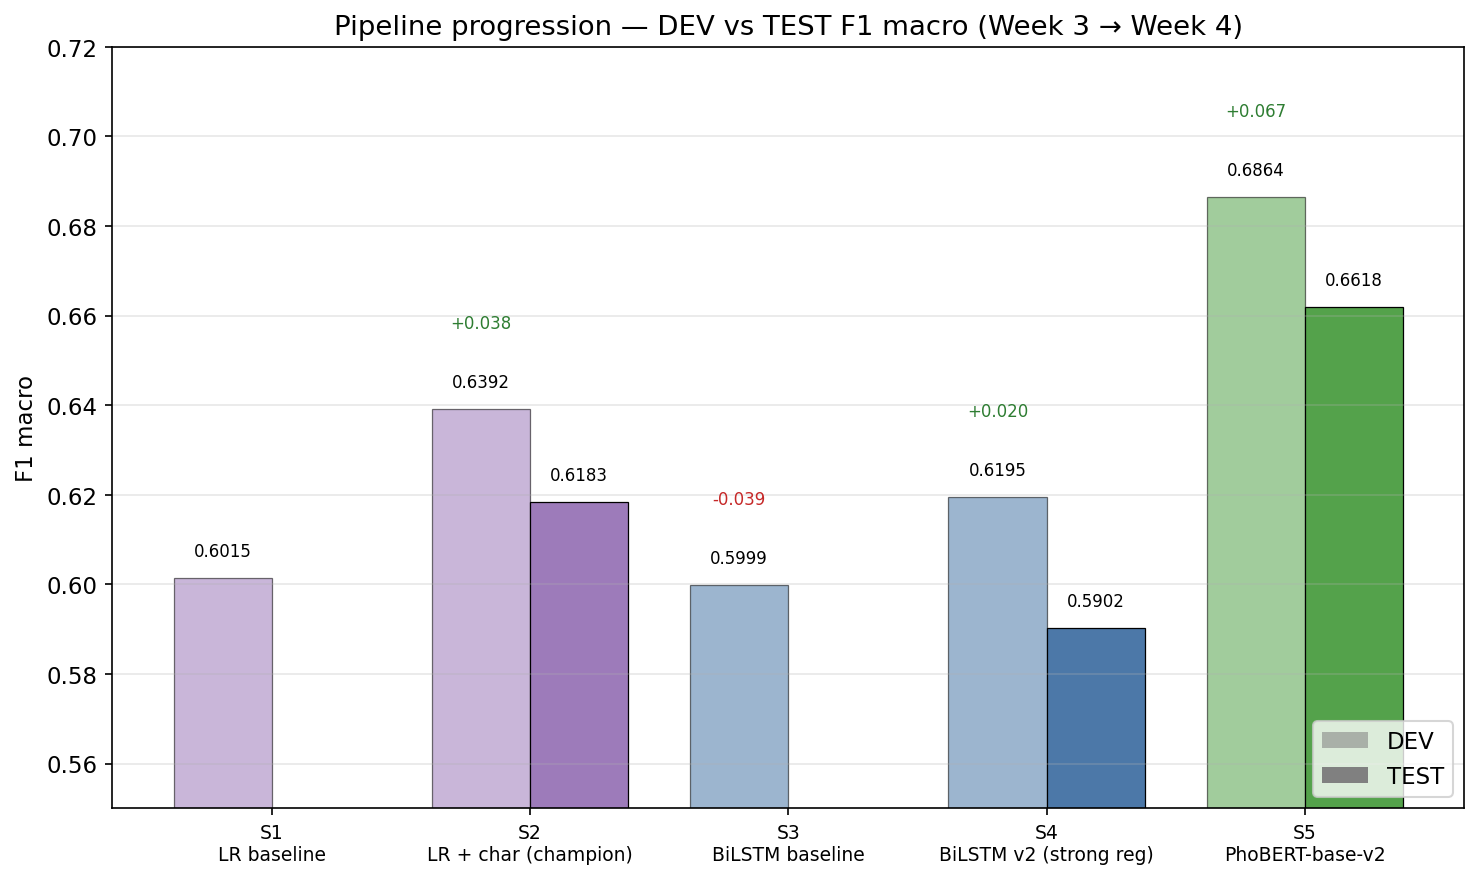
\includegraphics[width=0.95\linewidth]{F1_pipeline_progression.png}
\caption{Pipeline progression --- dev vs.\ test macro-F1 across the five
stages. Light bars = dev, dark bars = test. Annotations between
consecutive dev bars show the absolute improvement at each step.}
\label{fig:pipeline}
\end{figure}

\begin{figure}[H]
\centering
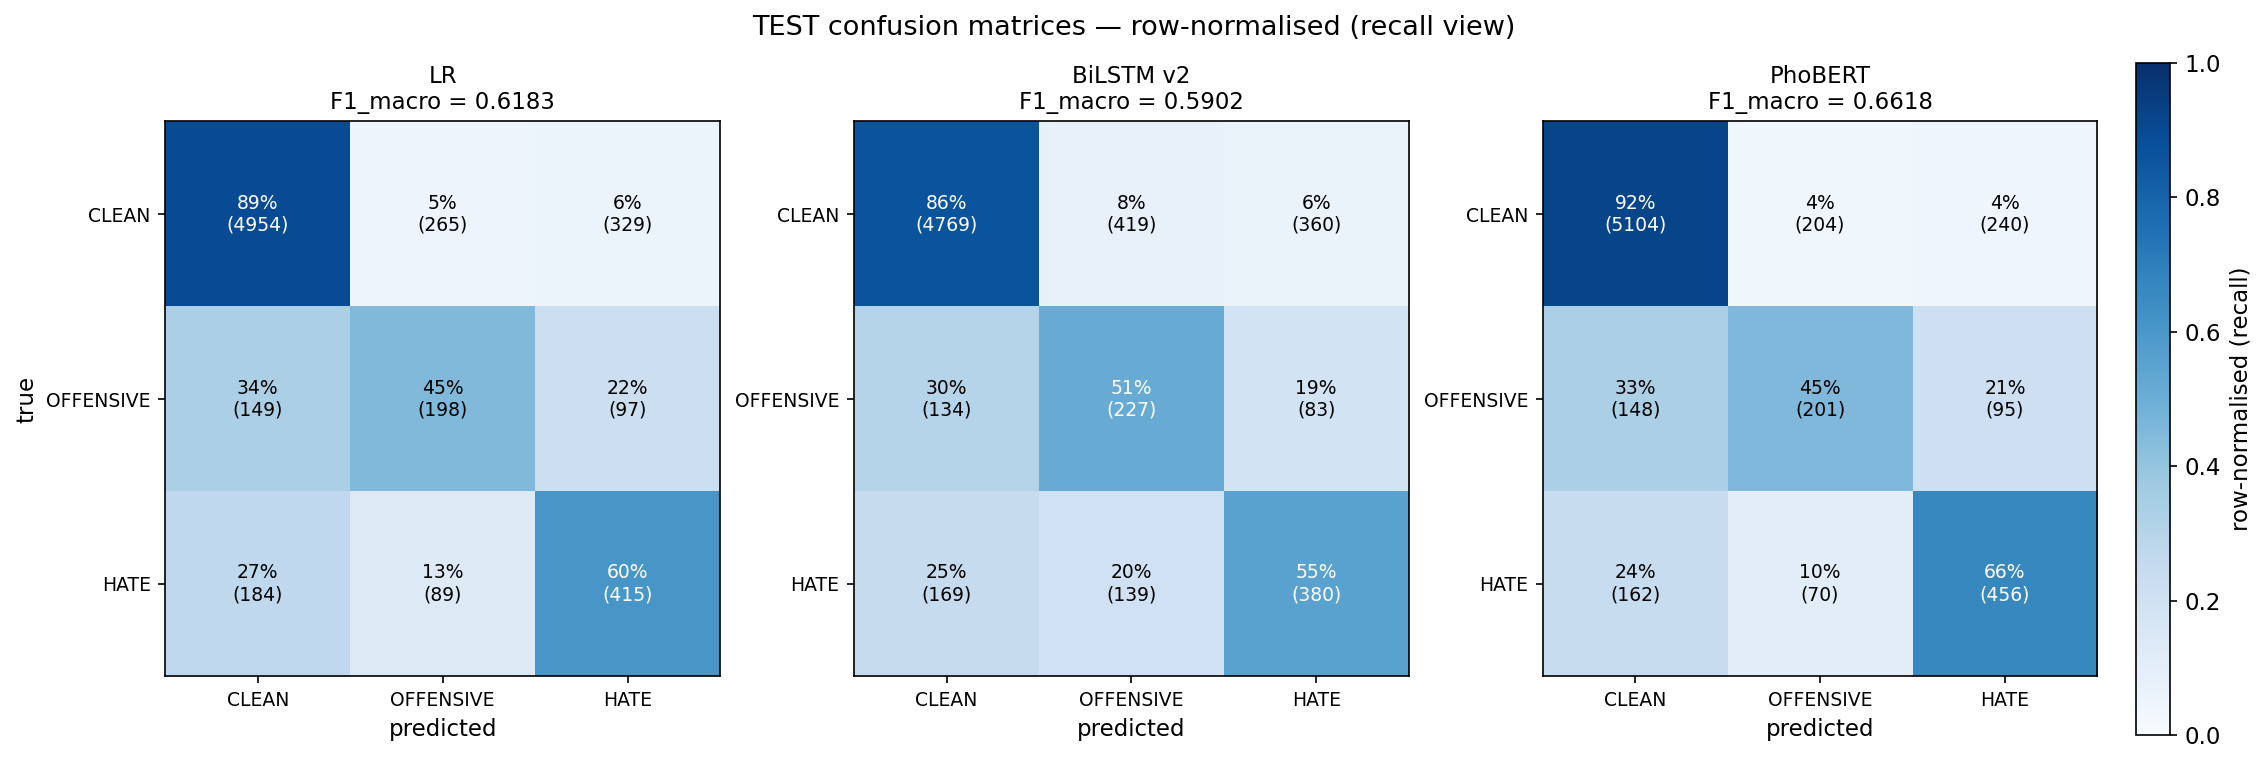
\includegraphics[width=0.95\linewidth]{F2_confusion_matrices.png}
\caption{Confusion matrices on test (row-normalised; diagonal = recall).
Both LR and PhoBERT route $\sim$33\% of OFFENSIVE samples to CLEAN ---
the persistent failure pattern analysed in Chapter~\ref{ch:errors}.}
\label{fig:cm}
\end{figure}

\begin{figure}[H]
\centering
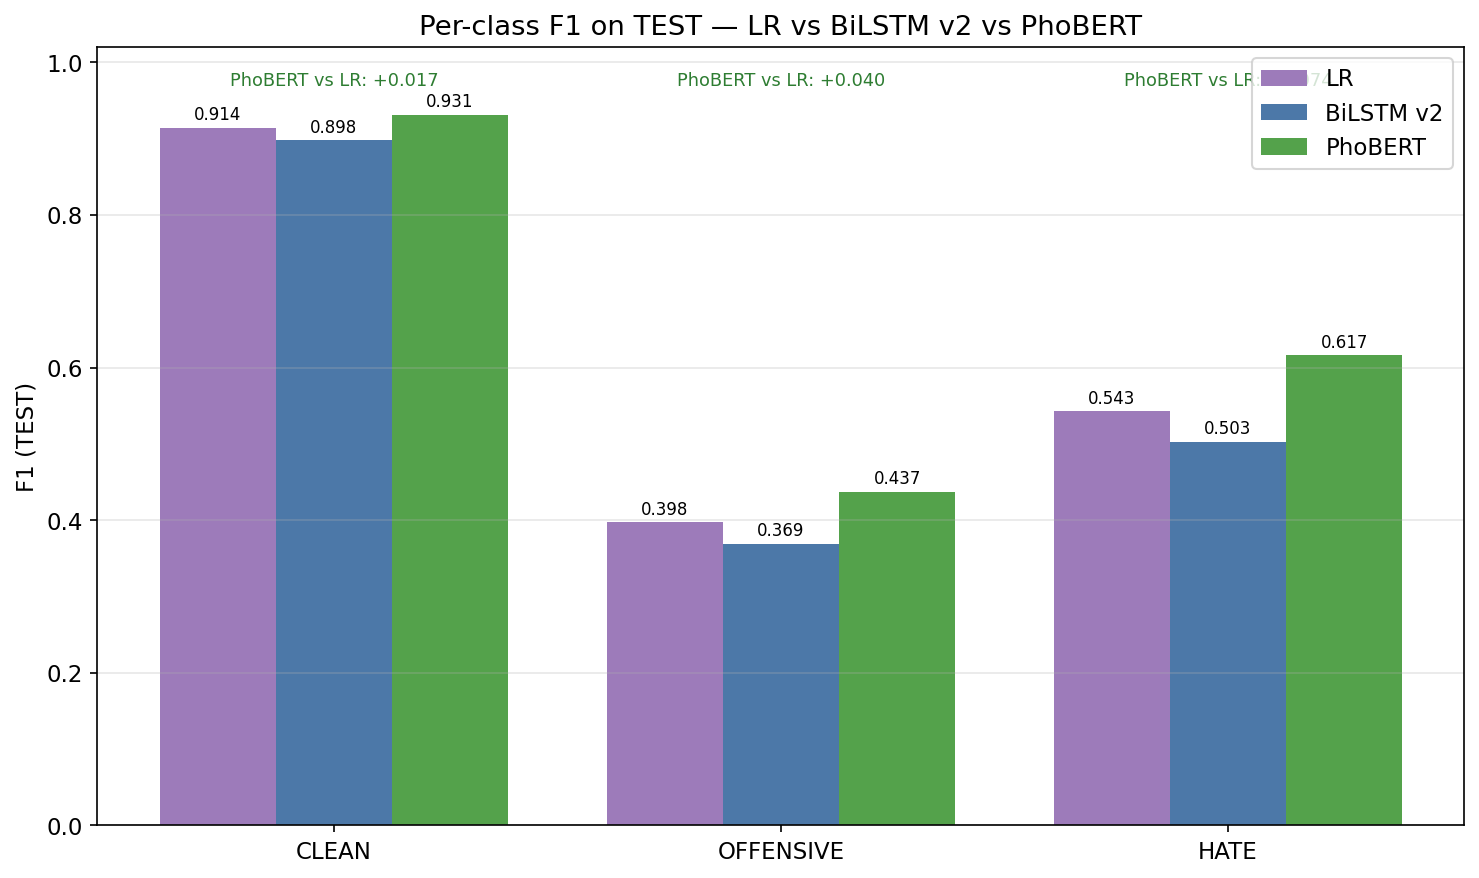
\includegraphics[width=0.95\linewidth]{F3_per_class_f1.png}
\caption{Per-class F1 on test. PhoBERT improves OFFENSIVE F1 by +0.040
and HATE F1 by +0.074 over the LR champion; CLEAN is already saturated.}
\label{fig:perclass}
\end{figure}

\subsection{PhoBERT Dev--Test Generalisation}
PhoBERT's dev$\rightarrow$test gap is $-0.0246$ ($-3.59\%$ relative) ---
``good generalisation with a mild gap'' by conventional thresholds
(Table~\ref{tab:devtest}). The single concerning row is OFFENSIVE F1,
which drops $-0.0760$ ($-14.80\%$ relative); this primes
Chapter~\ref{ch:errors}.

\begin{table}[H]
\centering
\caption{PhoBERT dev vs.\ test on the same checkpoint.}
\label{tab:devtest}
\begin{tabular}{lrrrr}
\toprule
Metric & Dev & Test & $\Delta$ abs.\ & $\Delta$ rel.\ \\ \midrule
F1\_macro     & 0.6864 & 0.6618 & -0.0246 & -3.59\% \\
F1\_CLEAN     & 0.9341 & 0.9312 & -0.0029 & -0.31\% \\
F1\_OFFENSIVE & 0.5134 & 0.4374 & -0.0760 & -14.80\% \\
F1\_HATE      & 0.6116 & 0.6166 & +0.0050 & +0.82\% \\
Accuracy      & 0.8645 & 0.8624 & -0.0021 & -0.24\% \\ \bottomrule
\end{tabular}
\end{table}

\subsection{Cost--Benefit Analysis}
PhoBERT's $+0.0435$ macro-F1 gain over LR costs roughly $865\times$
more training time (1732\,s vs.\ 2\,s) and $5400\times$ more parameters
(135M vs.\ 25k). For high-throughput production (millions of comments
per day) the LR champion remains attractive; PhoBERT is the right
default when latency budget allows ($\sim$22\,ms per sample on GPU with
fp16), with LR as a fallback or a coarse filter.

% =====================================================================
\chapter{Error Analysis}
\label{ch:errors}

\section{Quantitative Analysis}
\label{sec:quantitative}

\subsection{Cross-Model Disagreement Sets}
We define five disagreement subsets over the test set
(\texttt{notebooks/05a\_quantitative\_errors.ipynb}):
\textbf{A} (LR right, PhoBERT wrong; 303 cases),
\textbf{B} (PhoBERT right, LR wrong; 497 cases),
\textbf{C} (BiLSTM right, PhoBERT wrong),
\textbf{D} (all three wrong; 517 cases), and
\textbf{E} (all three right). Subset~D is the most analytically valuable
--- when three architecturally distinct models all fail in agreement,
the cause is more likely the input or the label than the model.

\subsection{Length Stratification --- a Counter-Intuitive Result}
\label{sec:length}
Stratifying the test set into five length buckets
(Figure~\ref{fig:length}) shows that the popular ``short comments are
harder'' hypothesis is \emph{inverted} on ViHSD: short comments are the
\textbf{easiest} bucket (F1 $\approx$ 0.71), and very long comments are
the hardest. More striking, PhoBERT's OFFENSIVE F1 collapses from
$\sim$0.60 on short comments to $\sim$0.03 on very long ones, while
HATE F1 increases. We interpret this as long comments diluting the
offensive signal --- a long comment that contains a mild insult is more
often labelled CLEAN by ViHSD annotators, but the model still picks up
the insult and over-escalates.

\begin{figure}[H]
\centering
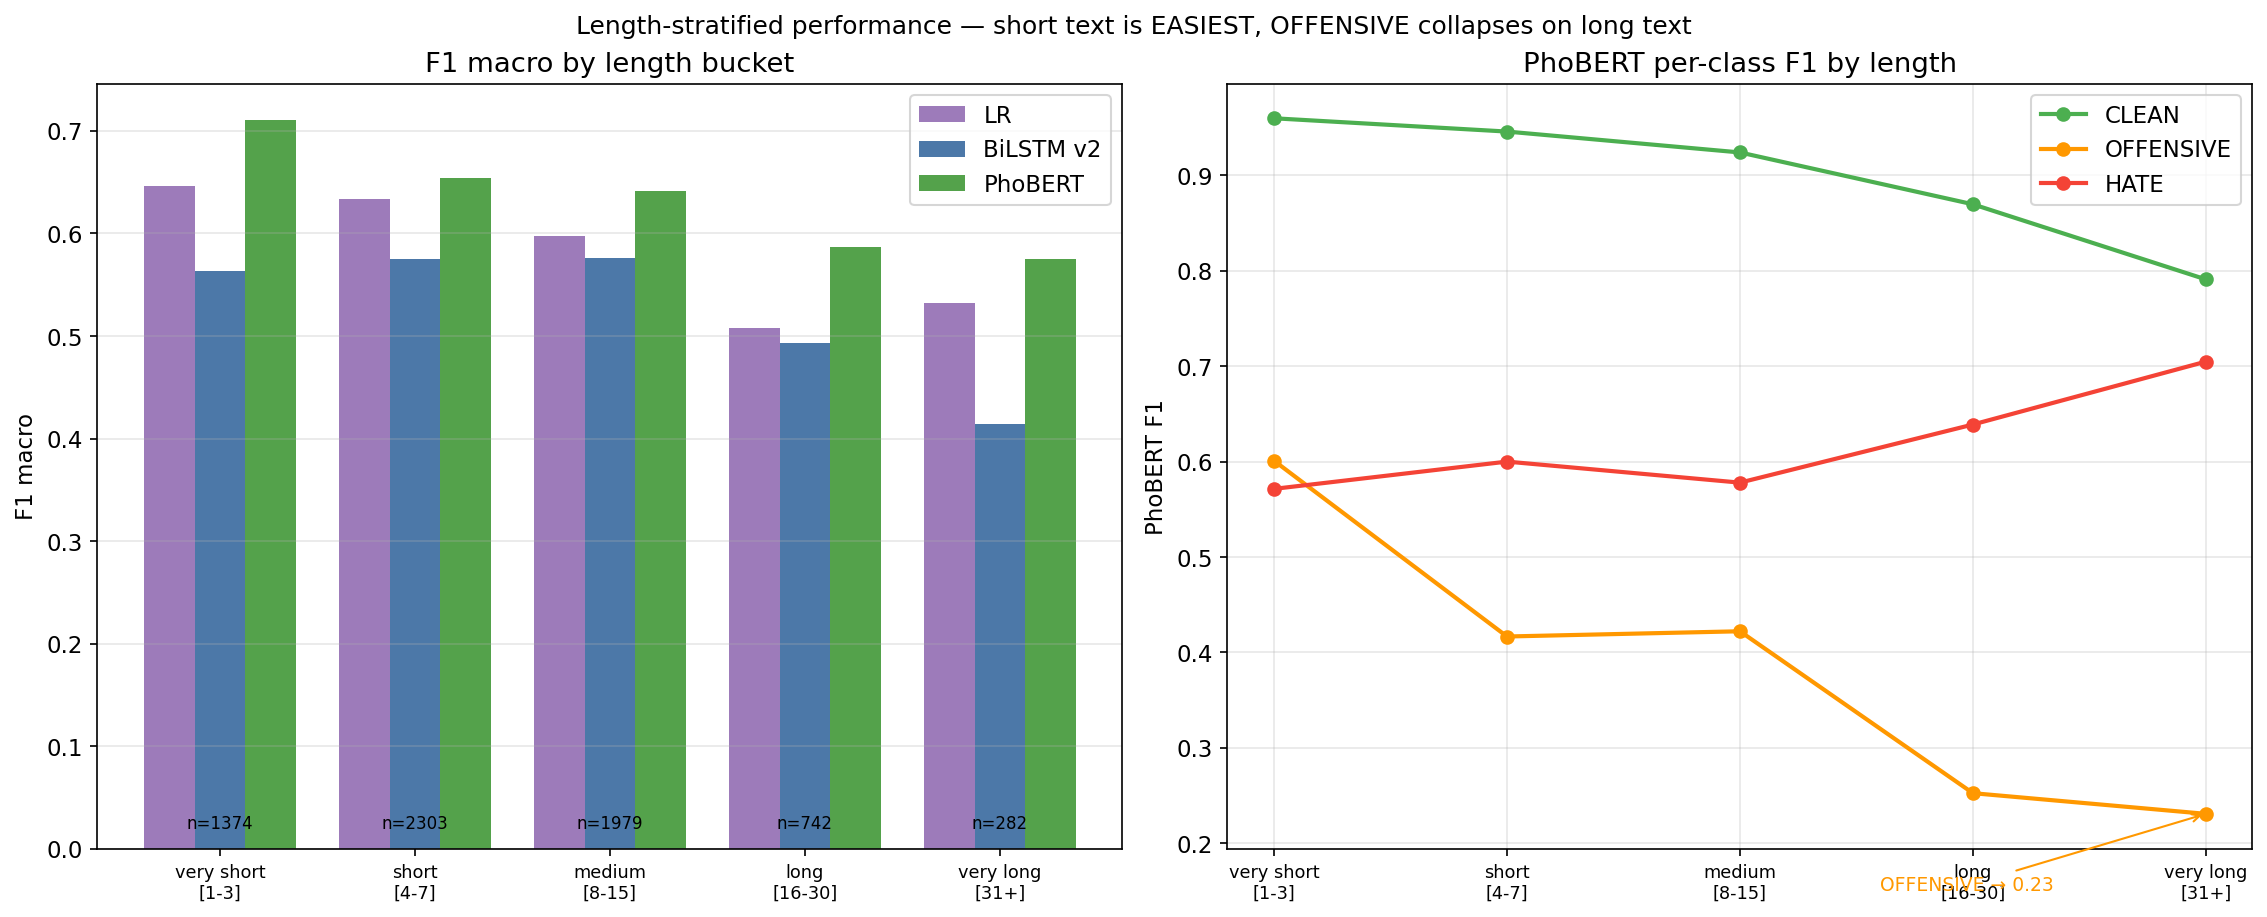
\includegraphics[width=0.95\linewidth]{F4_length_stratified.png}
\caption{Length-stratified test performance.
Left: macro-F1 by bucket for LR, BiLSTM, and PhoBERT.
Right: PhoBERT per-class F1 --- OFFENSIVE collapses on long comments
while HATE moves the opposite way.}
\label{fig:length}
\end{figure}

\subsection{Confidence Calibration}
PhoBERT's softmax output is \textbf{over-confident}
(Figure~\ref{fig:calib}). The Expected Calibration Error (ECE) on test
is 0.106; wrong predictions have a mean confidence of $\sim$0.83 and a
non-trivial mass at conf $> 0.9$. Raw softmax is therefore unsafe as an
auto-moderation threshold; temperature scaling or a human-in-the-loop
review queue for mid-confidence cases is required.

\begin{figure}[H]
\centering
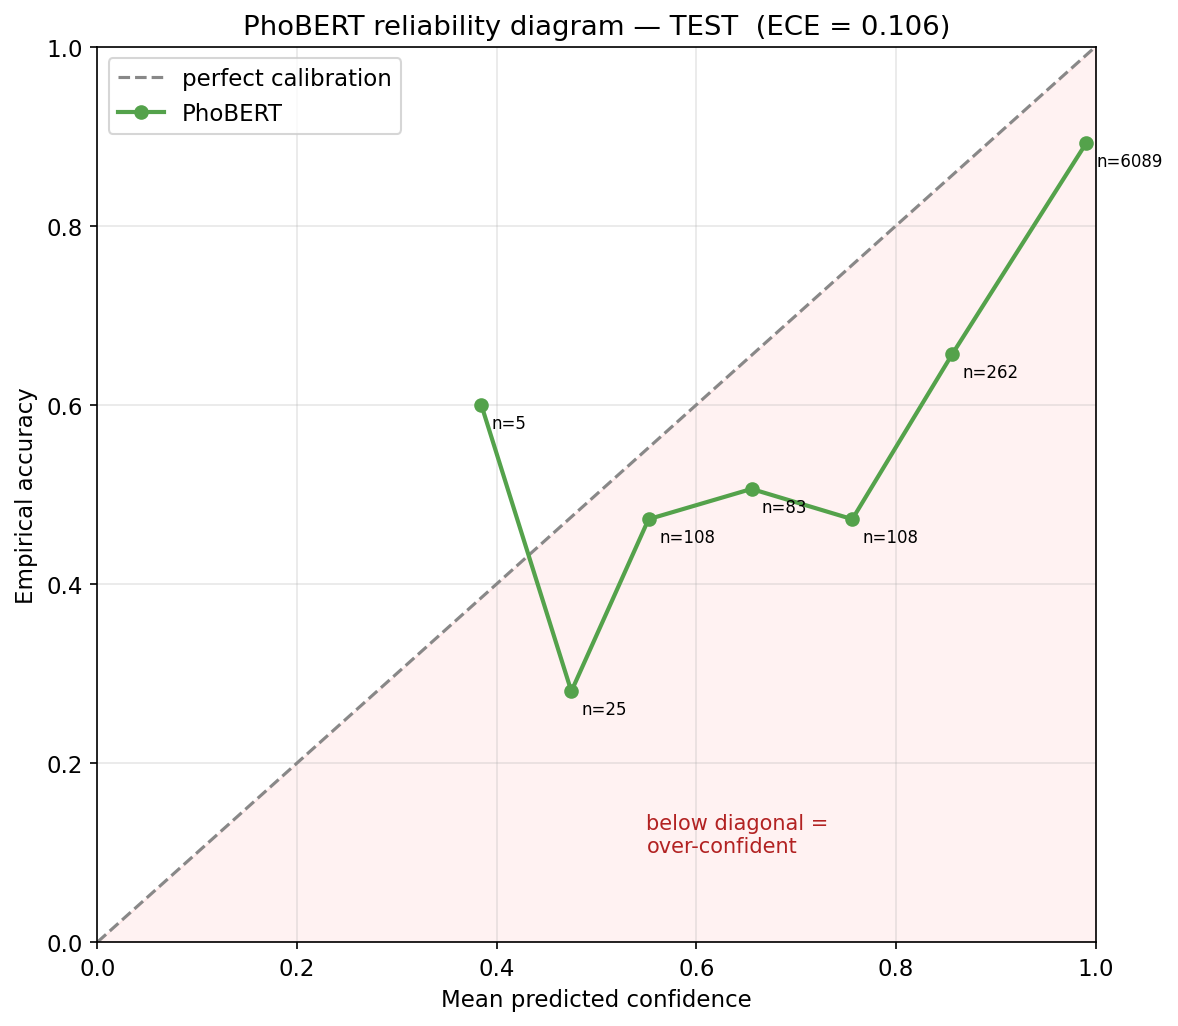
\includegraphics[width=0.7\linewidth]{F6_calibration.png}
\caption{PhoBERT reliability diagram on test. Most bins sit below the
diagonal, indicating systematic over-confidence. ECE = 0.106.}
\label{fig:calib}
\end{figure}

\section{Qualitative Analysis}
\label{sec:qualitative}
Building on the quantitative pass, we manually tag $n = 98$ stratified
failure cases (30 from subset~D, 20 each from A, B, and high-confidence
wrongs, 10 from long OFFENSIVE) along eight non-exclusive categories:
\texttt{sarcasm, code\_switching, teen\_code, implicit\_contextual,
annotation\_doubt, very\_short, long\_context, no\_toxic\_vocab}.

\begin{table}[H]
\centering
\caption{Manual tagging frequencies ($n=98$).}
\label{tab:tag}
\begin{tabular}{lrr}
\toprule
Category & Count & \% of pool \\ \midrule
\texttt{implicit\_contextual} & 77 & 79\% \\
\texttt{annotation\_doubt}    & 70 & 71\% \\
\texttt{no\_toxic\_vocab}     & 59 & 60\% \\
\texttt{teen\_code}           & 19 & 19\% \\
\texttt{sarcasm}              &  5 &  5\% \\
\texttt{code\_switching}      &  1 &  1\% \\ \bottomrule
\end{tabular}
\end{table}

\begin{figure}[H]
\centering
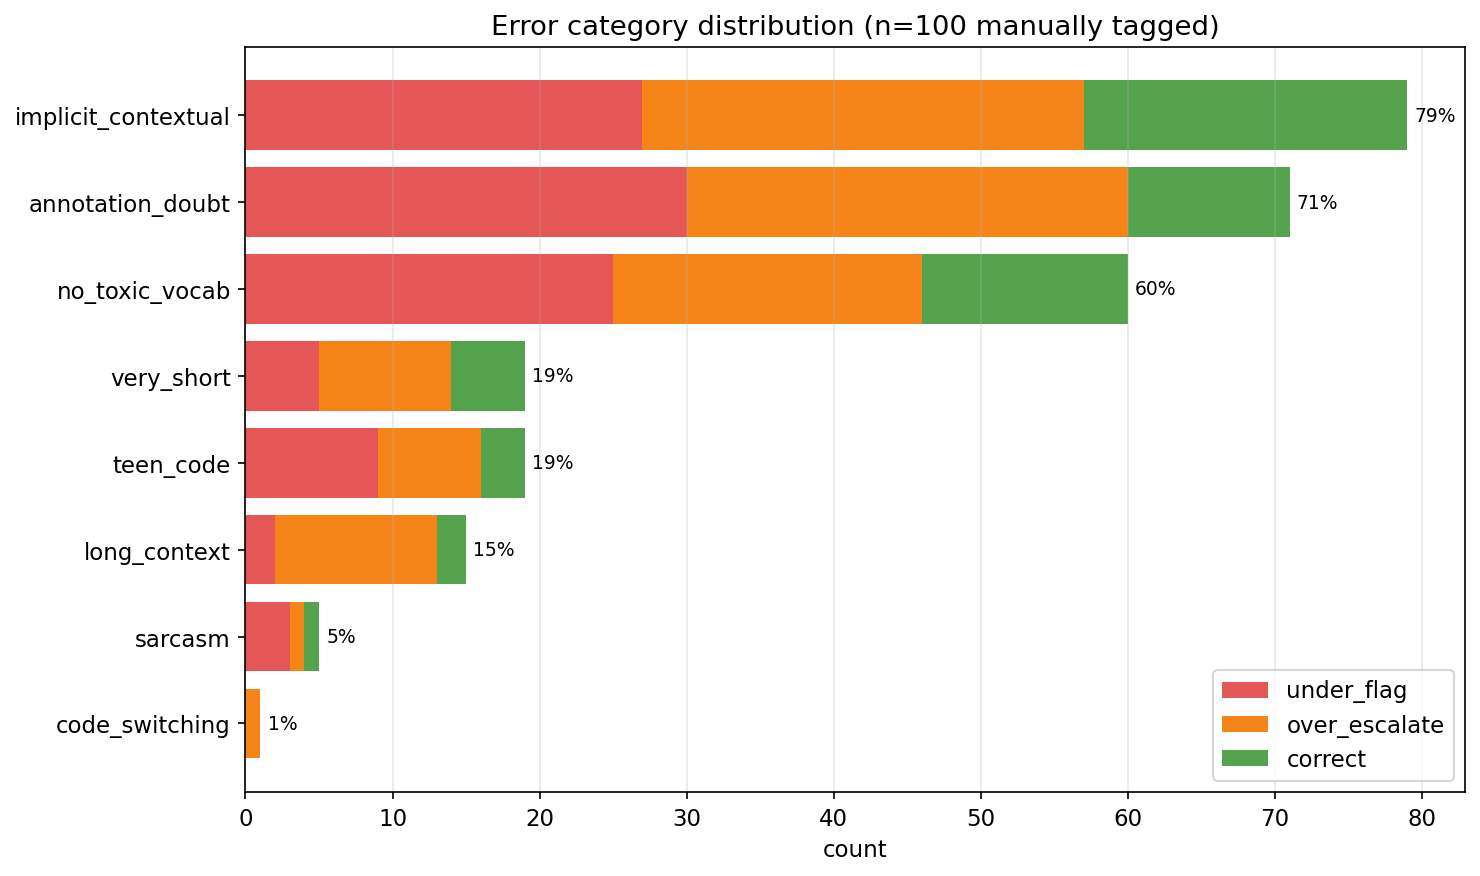
\includegraphics[width=0.95\linewidth]{F5_error_categories.png}
\caption{Error category distribution among 98 hand-tagged failures,
split by failure direction.}
\label{fig:errors}
\end{figure}

\section{Three-Tier Failure Framework}
\label{sec:framework}
From the tagging frequencies we propose the following deployment-oriented
framework for the residual error pool:

\begin{table}[H]
\centering
\caption{Three-tier failure framework with engineering levers.}
\label{tab:tiers}
\begin{tabular}{p{2.6cm} p{3.2cm} p{5.5cm}}
\toprule
Tier & Dominant category & Engineering lever \\ \midrule
1.\ Fixable          & \texttt{teen\_code} (19\%)            & Extend the teen-code / obfuscation dictionary in \texttt{src/preprocess.py}. Cheap; bounded gain. \\
2.\ Model-improvable & \texttt{implicit\_contextual} (79\%)   & Implicit-toxicity training data, target-aware features, larger or instruction-tuned models. \\
3.\ Fundamentally hard & \texttt{annotation\_doubt} (71\%) & Re-annotation with stricter guidelines, or adopt soft labels for the OFFENSIVE/HATE boundary. \\ \bottomrule
\end{tabular}
\end{table}

\section{Hypothesis Outcomes}
\label{sec:hypotheses}
We pre-registered four hypotheses before the qualitative pass:

\begin{table}[H]
\centering
\caption{Hypothesis outcomes after the error analysis.}
\label{tab:hypotheses}
\begin{tabular}{p{6.5cm} p{2.2cm} p{4cm}}
\toprule
Hypothesis & Outcome & Evidence \\ \midrule
H1 --- OFFENSIVE annotation ambiguity caps F1 & \textbf{Confirmed} &
\texttt{annotation\_doubt} 71\% overall, 83\% in subset D. \\
H2 --- Short comments are the hardest & \textbf{Refuted (inverted)} &
Short F1 $\approx$ 0.71 (best); very long F1 $\approx$ 0.58. \\
H3 --- Code-switching drives a major failure mode & \textbf{Refuted} &
\texttt{code\_switching} only 1\% of tagged failures. \\
H4 --- PhoBERT is over-confident on its mistakes & \textbf{Confirmed} &
ECE = 0.106, wrong-prediction mean conf $\approx 0.83$. \\ \bottomrule
\end{tabular}
\end{table}

The annotation ceiling (H1) is the highest-leverage finding: the
$\sim$30--34\% OFFENSIVE-to-CLEAN false-negative rate is essentially
constant across architectures (LR 33.6\%, BiLSTM v2 30.2\%, PhoBERT
33.3\%), suggesting an upper bound on achievable OFFENSIVE F1 around
$\sim$67--70\% \emph{given the current annotations}.

% =====================================================================
\chapter{Discussion}
\label{ch:discussion}

\section{Why does the annotation ceiling matter?}
A model-capacity story would predict that the more expressive model
(PhoBERT) sharply outperforms the simpler ones on the hardest class
(OFFENSIVE). The data shows otherwise: \emph{all three architectures}
under-flag $\sim$30--34\% of true OFFENSIVE samples. When three models
with vastly different inductive biases agree, the simplest explanation
is that the input is ambiguous --- usually because the gold label
itself is borderline. This reframes the bottleneck from
``how much more model do we need?'' to ``how much can we still trust
the labels?''.

\section{Length, dilution, and deployment}
The OFFENSIVE F1 collapse on long comments is plausibly a dilution
effect: a long comment containing one mild insult is, by ViHSD
guidelines, often labelled CLEAN, but the model still picks up the
insult and predicts OFFENSIVE. For deployment this implies that the
review queue should over-sample long comments flagged as OFFENSIVE,
since both the false-positive rate and the human-disagreement rate are
elevated there.

\section{Calibration as a deployment constraint}
PhoBERT's overconfidence (ECE = 0.106) is a real operational risk.
Temperature scaling on a held-out calibration set, or routing all
predictions with $\max p \in [0.4, 0.8]$ to human review, are the
minimal mitigations. Naive softmax-threshold deployment is
not advisable.

\section{Static embeddings underperform on this distribution}
The BiLSTM-v2 result (test F1 = 0.5902, \emph{below} the 25k-parameter
LR baseline) is initially surprising but consistent with the
literature on small-data, imbalanced text classification: static
word embeddings (PhoW2V here) cannot adapt their representations to
the dev$\rightarrow$test distribution shift the way contextual
sub-word embeddings (PhoBERT) can. The strong regularisation that
made BiLSTM-v2 the dev winner did not transfer.

\section{Limitations}
\begin{itemize}
  \item Manual tagging $n = 98$ is small and uses a single annotator;
        no inter-annotator agreement is reported.
  \item Error categories are non-exclusive --- the percentages do not
        sum to 100\%.
  \item Length effects are correlational; class balance within length
        buckets is not controlled.
  \item Hyperparameter search for BiLSTM and PhoBERT was limited by
        a single 6\,GB GPU; a larger sweep might shift the
        BiLSTM-vs-LR ordering.
  \item Results are reported with a single random seed (42). Variance
        estimates from multiple seeds would strengthen the
        cross-model claims.
\end{itemize}

% =====================================================================
\chapter{Conclusion}
\label{ch:conclusion}

\section{Summary of Contributions}
This thesis built a reproducible Vietnamese hate-speech classification
pipeline spanning Logistic Regression, BiLSTM, and PhoBERT-base-v2 on
the ViHSD benchmark. PhoBERT is the test champion at macro-F1 = 0.6618,
beating the LR baseline by +0.0435 absolute. Beyond the headline number,
we provided an in-depth error analysis that surfaced an
\emph{annotation ceiling} ($\sim$30--34\% OFFENSIVE-to-CLEAN under-flag
across all three models), a counter-intuitive length-pattern inversion
(short comments easiest, OFFENSIVE F1 collapsing on long comments),
and quantified PhoBERT over-confidence (ECE = 0.106). The
three-tier failure framework prioritises re-annotation as the
highest-leverage next step --- not more model capacity.

\section{Future Work}
\begin{itemize}
  \item \textbf{Re-annotation}: collect a second annotator on the 70
        \texttt{annotation\_doubt} cases and report Cohen's $\kappa$;
        consider soft labels for the OFFENSIVE/HATE boundary.
  \item \textbf{Calibration}: temperature scaling and selective
        prediction for deployment.
  \item \textbf{Implicit toxicity}: augment the training set with
        target-aware examples (group, slur target) that PhoBERT
        currently misses.
  \item \textbf{Multi-seed reporting}: rerun PhoBERT and BiLSTM-v2
        with seeds $\{42, 1, 2, 3, 4\}$ and report variance.
  \item \textbf{Inference cost}: distil PhoBERT to a smaller student
        model for high-QPS deployment, comparing against the LR
        baseline on a Pareto frontier.
\end{itemize}

% =====================================================================
\printbibliography[heading=bibintoc]

% =====================================================================
\appendix
\chapter{Reproducibility Notes}
\label{app:repro}
\begin{itemize}
  \item Repository: \texttt{<repo URL>}; final branch
        \texttt{claude/focused-gates-ag3vZ}.
  \item Random seed: 42 (Python, NumPy, PyTorch, HuggingFace).
  \item Environment: PyTorch 2.6 + CUDA 12.4, transformers 4.4x,
        underthesea 6.x, scikit-learn 1.x.
  \item All notebook outputs are auto-generated from artefacts in
        \texttt{results/} via the synthesis notebook
        \texttt{notebooks/05c\_synthesis.ipynb}.
\end{itemize}

\chapter{Additional Examples}
\label{app:examples}
% TODO: include 10-15 representative tagged failure cases from
% results/disagreement_set_D_all_wrong.csv with a brief comment per case.

\end{document}
